\documentclass[11pt]{article}

\usepackage[margin=1in]{geometry}
\usepackage{amsmath,amssymb}
\usepackage{graphicx}
\usepackage{booktabs}
\usepackage{xcolor}
\usepackage{hyperref}
\usepackage{setspace}
\onehalfspacing
\graphicspath{{../slides/figs/}}

\title{Time to Build and the Macroeconomy\\[0.3em]\large Robustness: union wage setting}
\author{Samuel Zhao\\University of Chicago}
\date{\today}

\begin{document}
\maketitle

\noindent The main text fixes the nominal wage at its steady-state level for the whole horizon. This
note replaces the fixed wage with Rotemberg union wage setting, a standard sticky-wage block in New
Keynesian models, and re-solves every policy experiment. Everything else is unchanged: the monthly
calibration, fixed production lags, the shocks, the planner's problem (commitment, the zero lower
bound, eight free months), and the comparison with the economy without time to build.

\paragraph{Summary.}
\begin{itemize}
  \item With 12-month wage contracts, about the average duration in U.S.\ data, the results are almost
        identical to the fixed wage. The monthly wage barely moves (by less than 0.01\%).
  \item With much more flexible 3-month contracts, every qualitative result survives:
        \begin{itemize}
          \item after a productivity fall, the planner cuts to zero with time to build and hikes to
                25\% annualised without it;
          \item the zero bound binds after supply shocks with time to build, and after demand shocks
                without it;
          \item policy matters far more for supply shocks with time to build.
        \end{itemize}
        The ratio of gains is smaller, because flexible wages raise the gain without time to build.
  \item One result is specific to the fixed wage. With forward-looking unions, warning about a
        \emph{demand} shock has some value even without time to build, because news reaches the economy
        through wages. For supply shocks, warning still has value only with time to build.
\end{itemize}

% =====================================================================
\section{Union wage setting}

Households supply differentiated labour to unions, which set nominal wages. The elasticity of
substitution between labour types is $\varepsilon_w$, and changing a wage carries a utility cost of
$\frac{\phi_w}{2}(\pi^w_t-1)^2$, where $\pi^w_t\equiv W_t/W_{t-1}$ is gross wage inflation. An employment
subsidy offsets the steady-state wage markup, so the steady state is the same as in the main text. In
a symmetric equilibrium the union's first-order condition is the nonlinear wage Phillips curve
\begin{equation}\label{eq:wpc}
  \phi_w(\pi^w_t-1)\pi^w_t
  =\varepsilon_wL_tC_t^{-\sigma}\Bigl(\chi L_t^{\eta}C_t^{\sigma}-\frac{W_t}{P_t}\Bigr)
  +\beta\frac{\theta_{t+1}}{\theta_t}\,\phi_w(\pi^w_{t+1}-1)\pi^w_{t+1},
\end{equation}
with $W_{-1}=\bar W$ and $\pi^w_t=1$ after the horizon. Wage inflation is positive when the marginal rate
of substitution exceeds the real wage, and it depends on expected future wage inflation. Equation
\eqref{eq:wpc} replaces $W_t=\bar W$. The household's Euler equation, producers, the final-good firm and
market clearing are unchanged. Period welfare subtracts the adjustment cost. As $\phi_w\to\infty$ the
model becomes the fixed-wage economy; as $\phi_w\to0$ it becomes the flexible-wage economy.

\paragraph{Calibration.} We set $\varepsilon_w=10$ and choose $\phi_w$ so that the linearised slope of
\eqref{eq:wpc} matches a Calvo wage contract with average duration $d$ months:
\[
  \frac{\varepsilon_w\,\omega L C^{-\sigma}}{\phi_w}=\frac{(1-\theta_w)(1-\beta\theta_w)}{\theta_w(1+\varepsilon_w\eta)},
  \qquad \theta_w=1-\frac1d .
\]
We use $d=12$ months as the baseline, close to the average wage duration in U.S.\ microdata, and
$d=3$ months as a much more flexible alternative. The slopes are $3.7\times10^{-4}$ and
$8.0\times10^{-3}$ per month.

% =====================================================================
\section{Results}

Table~\ref{tab:gains} reports the gain from optimal policy in every experiment, and
Table~\ref{tab:impact} the optimal rate on impact and the share of the peg's loss that policy removes.
Figures~\ref{fig:tfp}--\ref{fig:exp} compare the paths.

\begin{table}[h]
  \centering
  \caption{Gain from optimal policy: fixed wage vs.\ union wages}\label{tab:gains}
  \small\setlength{\tabcolsep}{4.5pt}
  \begin{tabular}{lcccccc}
    \toprule
    & \multicolumn{3}{c}{time to build} & \multicolumn{3}{c}{no time to build} \\
    \cmidrule(lr){2-4}\cmidrule(lr){5-7}
    & fixed & union 12m & union 3m & fixed & union 12m & union 3m \\
    \midrule
    \multicolumn{7}{l}{\emph{3\% productivity fall}}\\
    Unexpected & 0.123 & 0.123 & 0.128 & 0.011 & 0.012 & 0.014 \\
    News 1 month ahead & 0.371 & 0.371 & 0.371 & 0.008 & 0.008 & 0.012 \\
    News 13 months ahead & 0.384 & 0.385 & 0.375 & 0.008 & 0.009 & 0.014 \\
    News 13 months ahead, policy from $t=0$ & 0.106 & 0.108 & 0.109 & 0.001 & 0.002 & 0.004 \\
    \midrule
    \multicolumn{7}{l}{\emph{1\% demand fall ($\times10^{-3}$)}}\\
    Unexpected & 2.18 & 2.19 & 2.43 & 3.65 & 3.70 & 4.64 \\
    News 1 month ahead & 2.68 & 2.73 & 3.46 & 3.65 & 3.76 & 5.37 \\
    News 13 months ahead & 2.36 & 2.81 & 3.91 & 3.65 & 4.17 & 6.22 \\
    News 13 months ahead, policy from $t=0$ & 1.09 & 1.42 & 1.77 & 0.33 & 0.70 & 1.39 \\
    \bottomrule
  \end{tabular}

  \medskip
  \parbox{0.95\textwidth}{\footnotesize Gain $=$ optimal $-$ peg, \% of one month's steady-state
  consumption, valued at $t=-13$. ``Union 12m'' and ``union 3m'': Rotemberg unions calibrated to 12- and
  3-month Calvo contracts.}
\end{table}

\begin{table}[h]
  \centering
  \caption{Optimal rate and share of the loss removed}\label{tab:impact}
  \footnotesize\setlength{\tabcolsep}{3.5pt}
  \begin{tabular}{llcccccc}
    \toprule
    & & \multicolumn{3}{c}{time to build} & \multicolumn{3}{c}{no time to build} \\
    \cmidrule(lr){3-5}\cmidrule(lr){6-8}
    & & fixed & union 12m & union 3m & fixed & union 12m & union 3m \\
    \midrule
    Productivity & $i_0$, unexp. & 0.0 & 0.0 & 0.0 & 24.9 & 24.9 & 24.9 \\
    & share, unexp. & 31\% & 31\% & 32\% & 100\% & 100\% & 100\% \\
    & $i_{-1}/i_0$, 13m & 25.4/0.0 & 25.1/0.0 & 23.3/0.0 & 0.0/15.0 & 0.0/15.0 & 0.0/14.1 \\
    & share, 13m & 54\% & 54\% & 52\% & 67\% & 71\% & 77\% \\
    \midrule
    Demand & $i_0$, unexp. & 2.5 & 2.5 & 2.5 & 0.0 & 0.0 & 0.0 \\
    & share, unexp. & 100\% & 100\% & 100\% & 77\% & 77\% & 80\% \\
    & $i_{-1}/i_0$, 13m & 4.9/2.6 & 4.9/2.6 & 4.9/2.6 & 12.6/0.0 & 12.5/0.0 & 12.1/0.0 \\
    & share, 13m & 100\% & 100\% & 100\% & 77\% & 79\% & 84\% \\
    \bottomrule
  \end{tabular}

  \medskip
  \parbox{0.95\textwidth}{\footnotesize Rates annualised (steady state 4\%). ``Unexp.'': unexpected
  shock. ``13m'': shock announced 13 months ahead, policy from the news date. ``Share'': share of the
  peg's loss relative to the flexible wage removed by optimal policy.}
\end{table}

\paragraph{Twelve-month contracts.} The monthly wage barely moves: by less than 0.01\% after a 3\%
productivity fall. With time to build, every productivity gain and optimal rate is within 2\% of the
fixed-wage value. Without time to build, the gains are two orders of magnitude smaller, and the union
moves them more in relative terms. For example, with policy acting only from the shock date the gain is
0.002 against 0.001; with 13 months of warning it is 0.009 against 0.008. For demand shocks with news,
the gains are somewhat larger than with the fixed wage (for example $2.8$ against $2.4\times10^{-3}$ at
13 months, with time to build). Over a long warning period, unions move
wages in anticipation even with sticky contracts, which makes the peg worse. The optimal rate path is
the same: evaluated in the fixed-wage model, the union optimum gives the same welfare as the
fixed-wage optimum.

\paragraph{Three-month contracts.} The comparison with time to build is unchanged where it matters:
\begin{itemize}
  \item \emph{Sign of the response.} After an unexpected productivity fall, the optimal rate is still
        cut to zero with time to build and raised to 25\% annualised without it.
  \item \emph{Zero lower bound.} It still binds after the productivity shock with time to build, and
        for two months after the demand shock without it.
  \item \emph{Size of the gains.} With time to build the productivity gains hardly change (0.128
        unexpected and 0.375 with 13 months of warning). Without time to build they rise, from 0.011 to
        0.014. The ratio of gains falls from about 11 to 9 for unexpected shocks, and from 50 to 27 with
        13 months of warning. Flexible wages do some of the stabilising work that policy does in the
        fixed-wage economy, and they help more where policy had less to do.
  \item \emph{Demand shocks.} The gains rise with wage flexibility in both economies, and the ranking
        is unchanged: policy matters more for demand shocks without time to build.
\end{itemize}

\paragraph{Warning and commitment.} For productivity shocks, warning still has no value without time
to build at either contract length (0.014 with no warning, 0.012 with one month and 0.014 with
thirteen, for 3-month contracts). For demand shocks it does once wages are forward-looking: without time
to build, the gain rises from $4.6$ to $6.2\times10^{-3}$ with 13 months of warning under 3-month
contracts. The main text's statement that warning matters only through firms' production plans
therefore holds for supply shocks in general, and for demand shocks with a rigid wage.

The commitment exercise, which locks production as if the shock were unexpected, gives:
\begin{itemize}
  \item productivity, 12-month contracts: 0.1227 (one month of warning) and 0.1229 (13 months),
        against 0.1228 with no warning;
  \item demand: $2.21$ and $2.31\times10^{-3}$ against $2.19\times10^{-3}$.
\end{itemize}
With union wages, expectations alone are worth something, through wages, but only a few per cent of the
gain. Firms' re-planning is still almost all of it.

\begin{figure}[h]
  \centering
  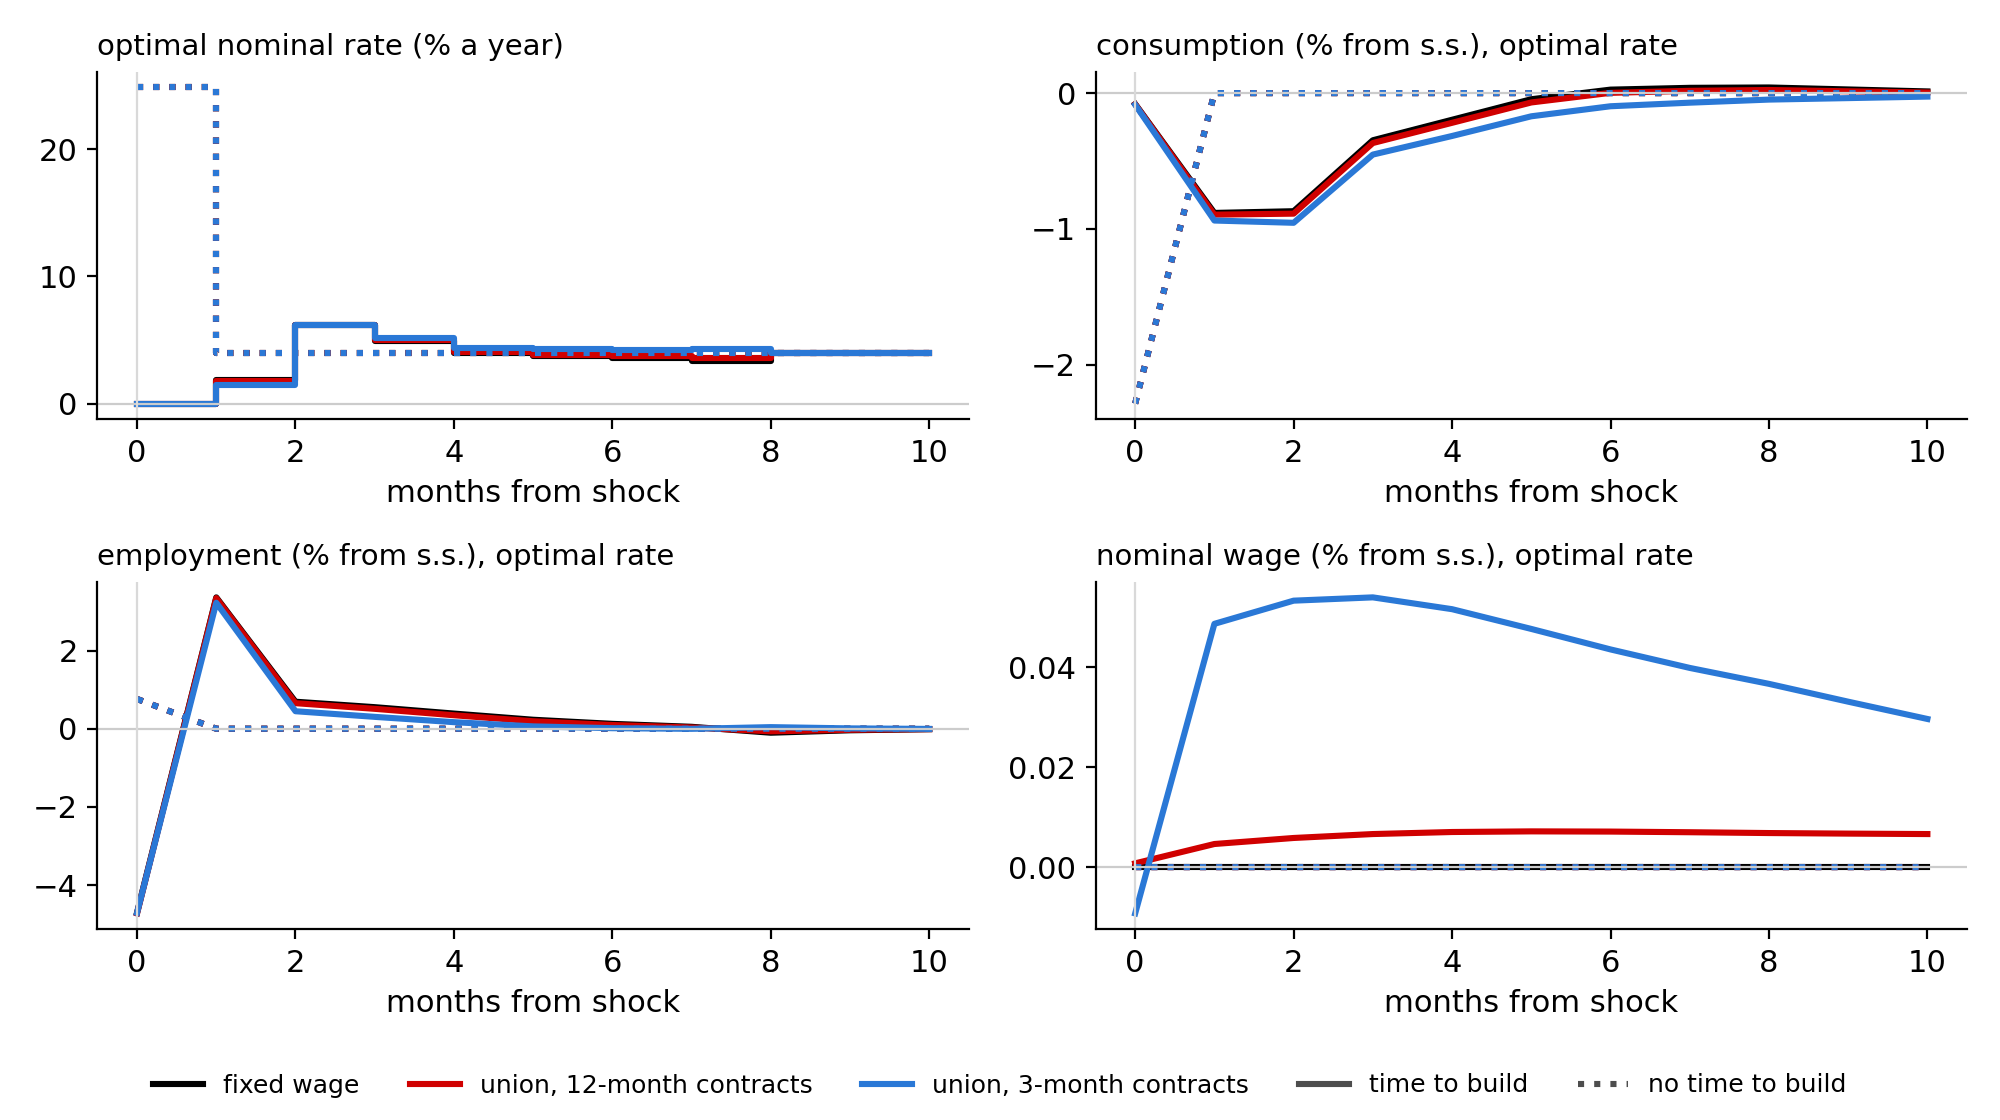
\includegraphics[width=\textwidth]{uw_unexp_tfp.png}
  \caption{Unexpected 3\% productivity fall under the optimal rate: fixed wage (black), unions with
  12-month (red) and 3-month (blue) contracts. Solid: time to build; dotted: no time to build.}
  \label{fig:tfp}
\end{figure}

\begin{figure}[h]
  \centering
  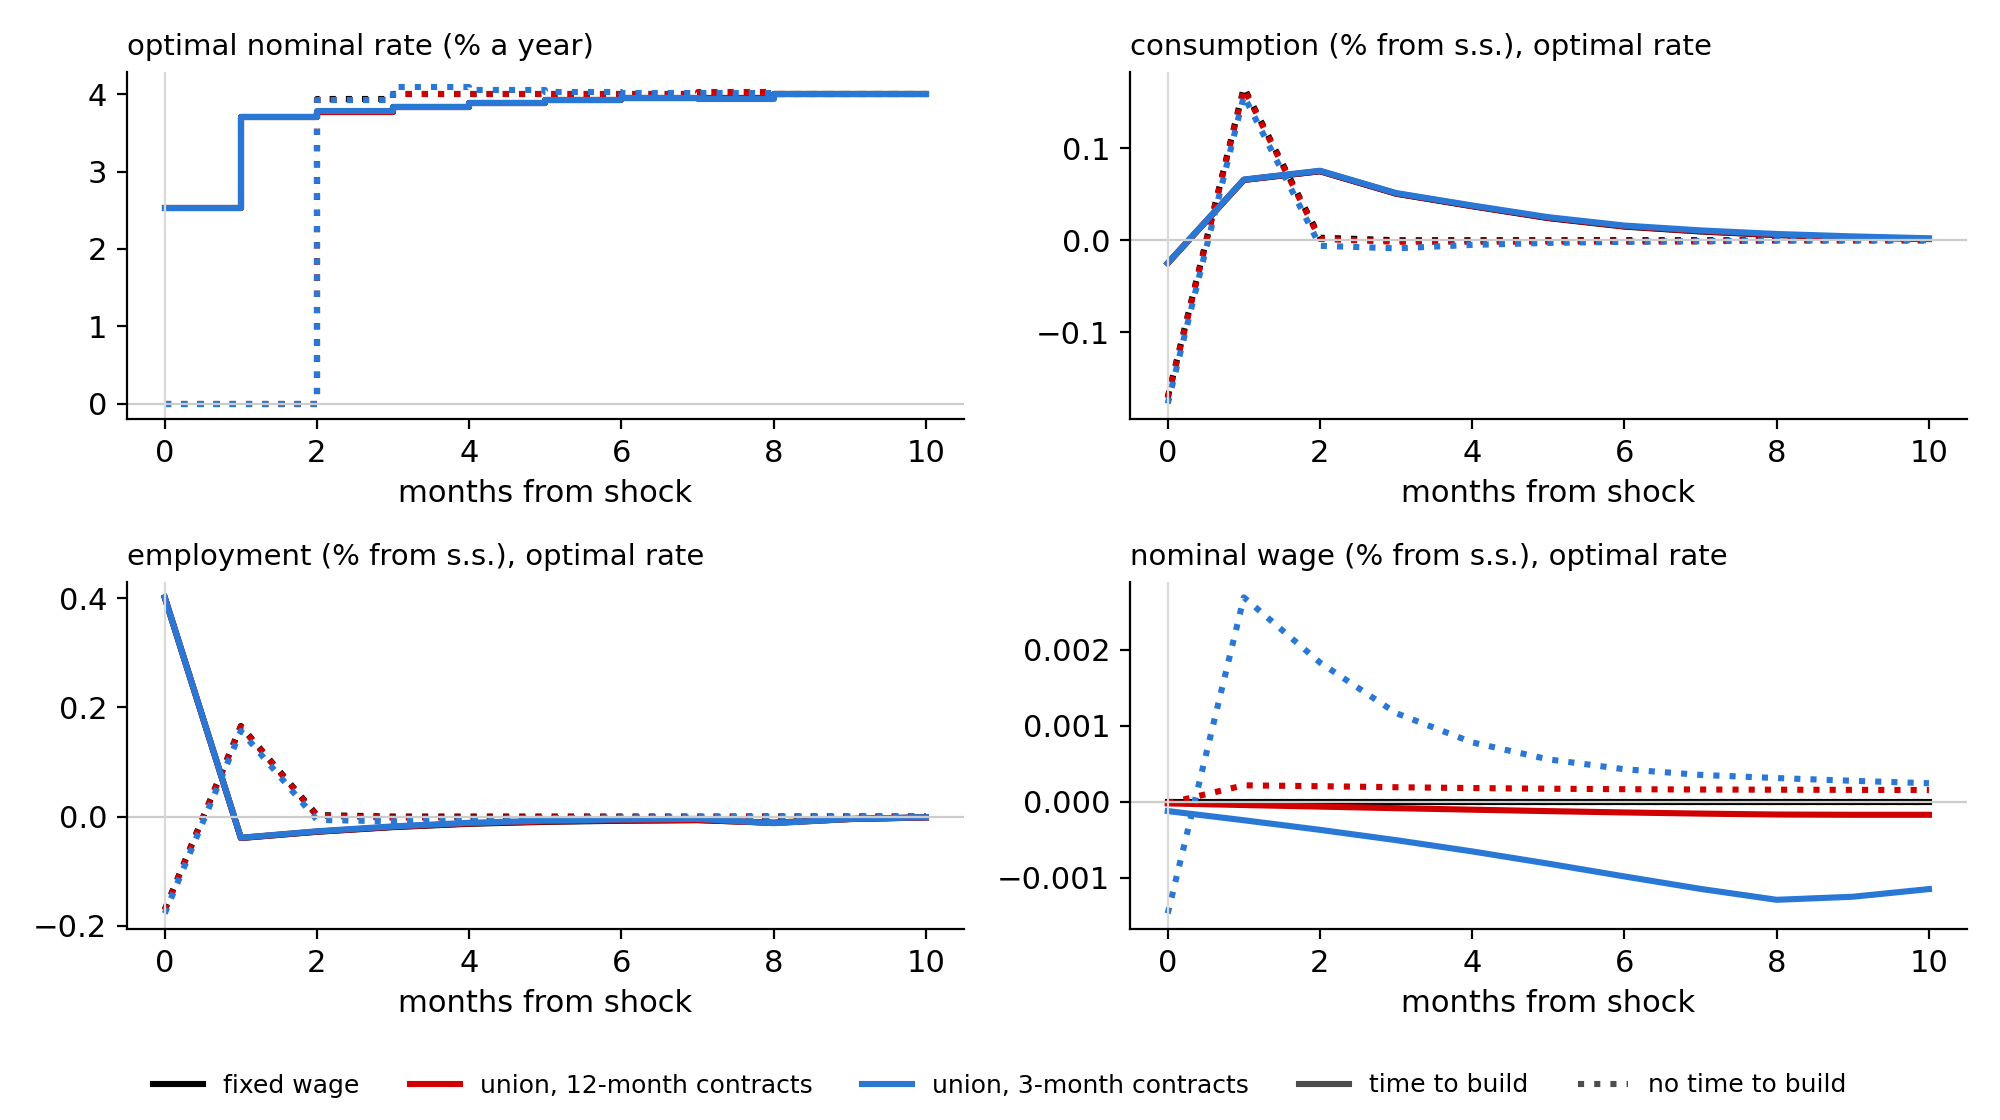
\includegraphics[width=\textwidth]{uw_unexp_dem.png}
  \caption{Unexpected 1\% demand fall under the optimal rate. Same lines as Figure~\ref{fig:tfp}.}
  \label{fig:dem}
\end{figure}

\begin{figure}[h]
  \centering
  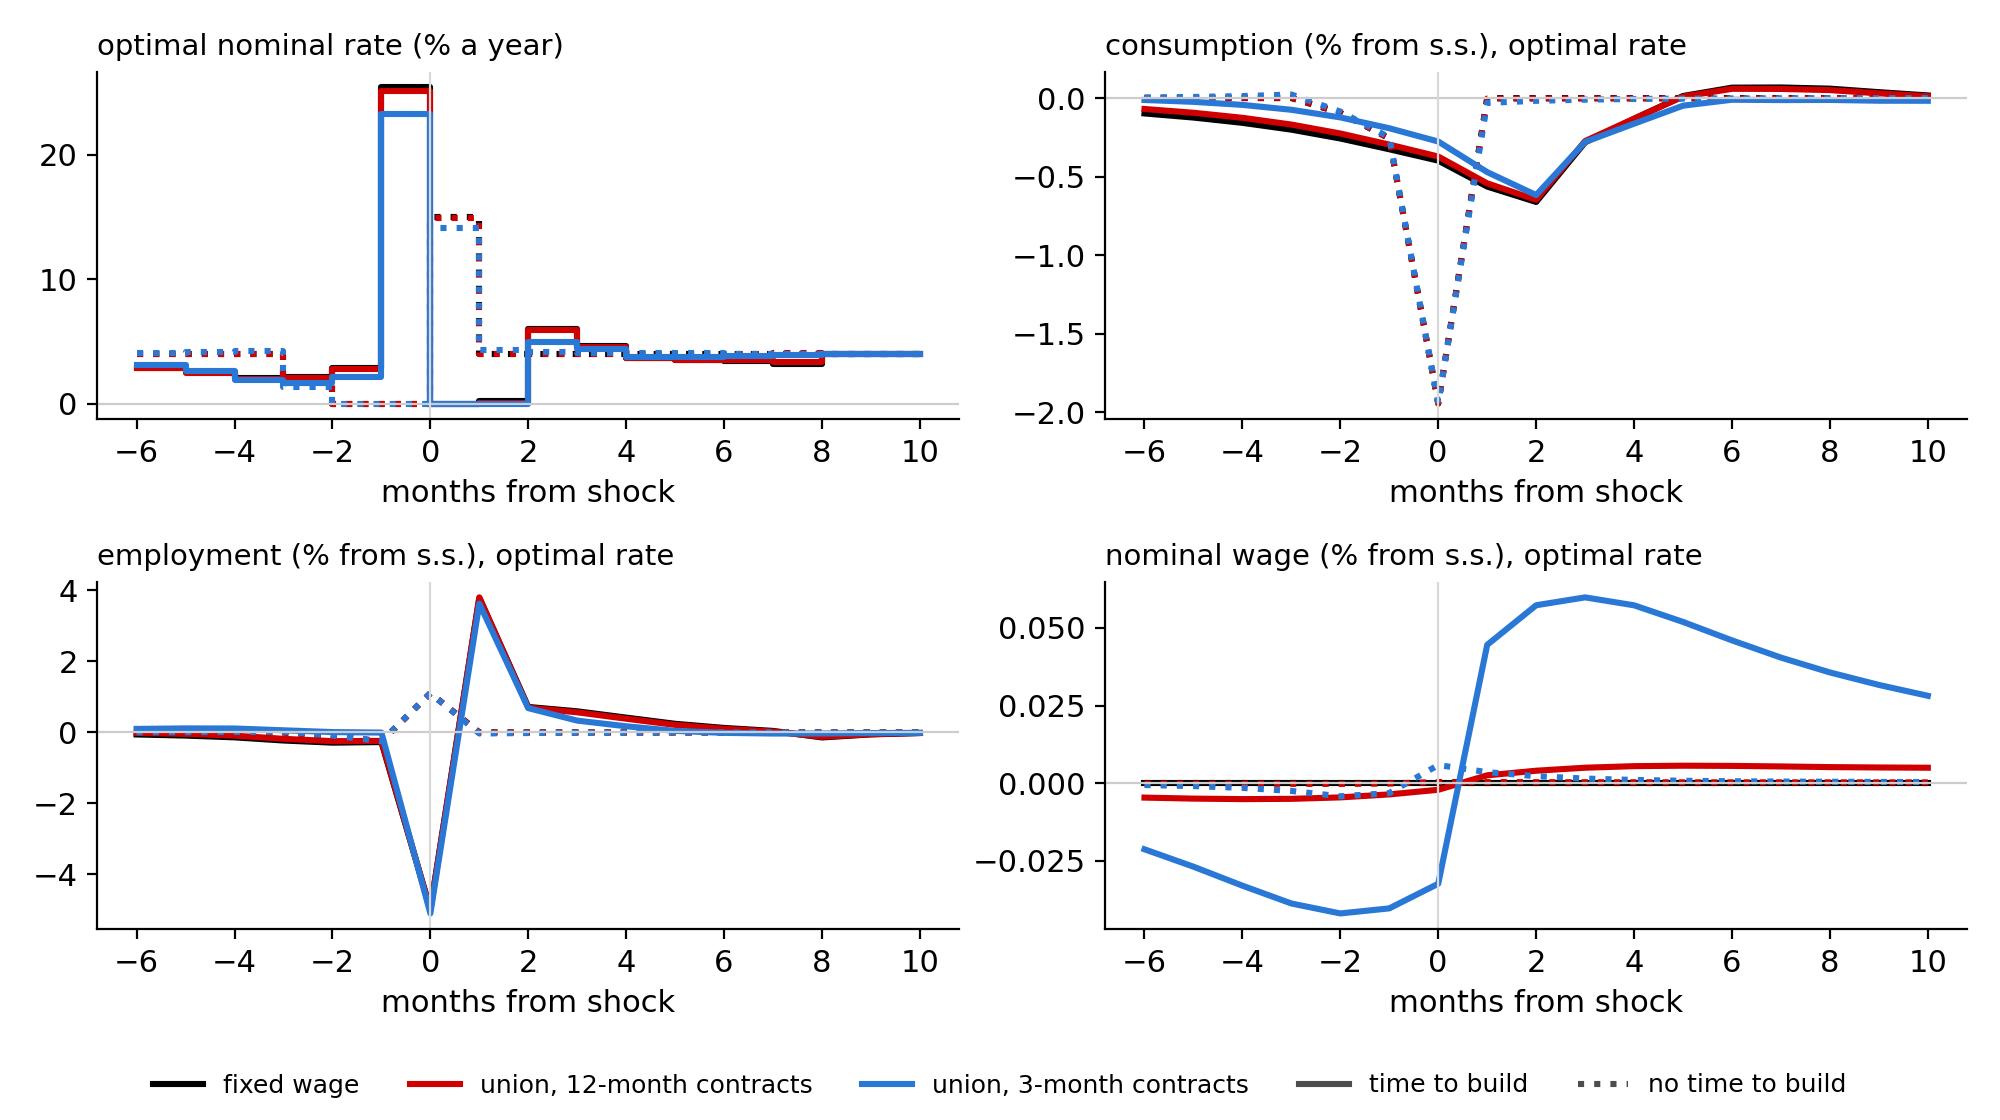
\includegraphics[width=\textwidth]{uw_exp_tfp.png}
  \caption{3\% productivity fall announced 13 months ahead, policy from the news date. Same lines as
  Figure~\ref{fig:tfp}.}
  \label{fig:exp}
\end{figure}

\end{document}
